\documentclass[12pt]{report}

\usepackage[utf8]{inputenc}
\usepackage{listings}
\usepackage{algpseudocode}	 % pseudo code
\usepackage{graphicx}		 % graphics
\usepackage{amsmath}		 % math symbols
\usepackage{amssymb}		 % math symbols
\usepackage[colorlinks,      % hyperlinks
            linktocpage,
            linkcolor=black,
            urlcolor=black]
            {hyperref}

\graphicspath{{images/}}

% COMMANDS
% ----------------------------------------------------------------
\newcommand{\answer}{\textbf{A:}}
\newcommand{\TITLE}{\Large\textbf{DBS:} Exercise 2}
\newcommand{\AUTHOR}{\normalsize{John Nguyen, Gavithishan Ravechandran}}
\newcommand{\TUTOR}{\normalsize{Tutor: Christian Hofmann (Thur 12pm)}}

% DOCUMENT
% ----------------------------------------------------------------
\begin{document}

\noindent\TITLE \hfill 5/5/17\\[3pt]
\TUTOR\\
\AUTHOR\\
\rule{\textwidth}{0.4pt}\\

\section*{1. Aufgabe: Grundlagen}

\begin{enumerate}
\item[(4 P)] Geben Sie zwei Beispiele für einen Entitätstypen an.
\item[\answer]
  One example entity type is user profile on a social networking site, that relates data about a single user. Another example is a rental car belong to a rental service

\item[(4 P)] Geben Sie zwei Beispiele für ein Attribut an.
\item[\answer]
  Continuing with the user profile example, two attributes could be a) the email address used to create the profile and a username.

\item[(4 P)] Was ist ein Schlüsselattribut?
\item[\answer]
  A key attribute is an entity attribute that must have a unique value amount the entities it is asssociated to. Thus a key attribute can also be used to identify a single entity. In the example above, the email address would be a key attribute for the profile entity, as each email address should only be linked at most one single user profile.

\item[(2 P)] Geben Sie ein Beispiel für eine nicht-rekursive 1-zu-N Relation an.
\item[\answer]
  Consider the entity types a) Monkey, and b) Zoo, and the relationship type ``belongs to''. The relationship between the two entities is a 1-to-many relationship, because a monkey belongs to only one zoo, but a zoo may own many monkies.

\item[(2 P)] Geben Sie ein Beispiel für eine nicht-rekursive N-zu-M Relation an.
\item[\answer]
  Consider the entity types a) Book, and b) Person, and the relationship type ``authored by''. This is a many-to-many relationship because a book can have many authors, and person can have written many books.

\item[(4 P)] Geben Sie ein Beispiel für eine rekursive Relation an. Wie sieht es mit dem Kardinalitätsverhältnis Ihres Beispiels aus?
\item[\answer]
  Consider the entity type Person and the relationship type ``is a friend of''. This is a recursive relationship because a person is a friend of another person. The cardinality ratio is many-to-many, because each person can have multiple friends.

\end{enumerate}

\section*{2. Aufgabe: ER-Modellierung 1}
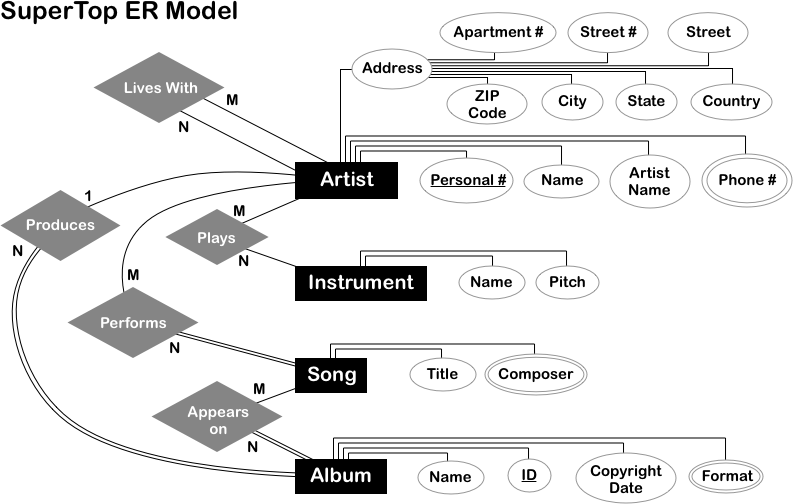
\includegraphics[scale = 0.7, angle = -90]{Q2}

% \begin{enumerate}
%
% \item[(25 P)] Erstellen Sie ein ER-Modell in einfacher Chen-Notation auf Grundlage der folgenden Beschreibung:
% Das Platten-Label SuperTop möchte Informationen über Musiker ihrer Alben sowie weitere Unternehmensdaten in einer Datenbank speichern. Jeder Musiker/Interpret, der Aufnahmen bei SuperTop gemacht hat, erhält eine Personennummer. Daneben werden noch Daten gespeichert wie Name, Künstlername, Adresse und Telefonnummer. Schlecht bezahlte Musiker teilen sich häufig eine Wohnung mit anderen Musikern. Jedes für Aufnahmen genutzte Instrument erhält einen Namen (Gitarre, Flöte, etc.) und eine Tonhöhe (c,d\#, etc.). Jedes Album hat einen Namen, eine ID, ein Copyright-Datum und ein oder mehrere Tonträgervarianten (CD, USB, etc.). Jedes aufgenommene Stück hat einen Titel und einen Komponisten. Jeder Musiker kann, muss aber nicht, ein oder mehrere Instrumente spielen. Ein Instrument kann auch durch mehrere Musiker gespielt werden. Jedes Album enthält eine bestimmte Anzahl an Stücken. Ein Stück kann auf mehreren Alben erscheinen. Jedes Stück wird durch einen oder mehrere Musiker gespielt. Ein Musiker kann mehrere Stücke spielen. Jedes Album hat einen Musiker, der als Produzent auftritt. Ein Musiker kann natürlich mehrere Alben produzieren.
% \end{enumerate}

\newpage

\section*{3. Aufgabe: ER-Modellierung 2}
\vspace{2cm}
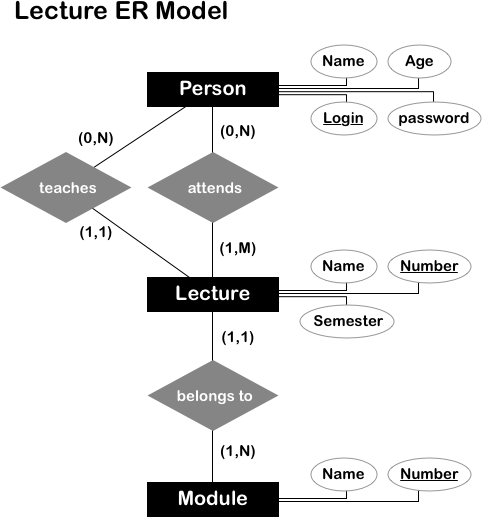
\includegraphics[scale = 0.7]{Q3a}
\newpage
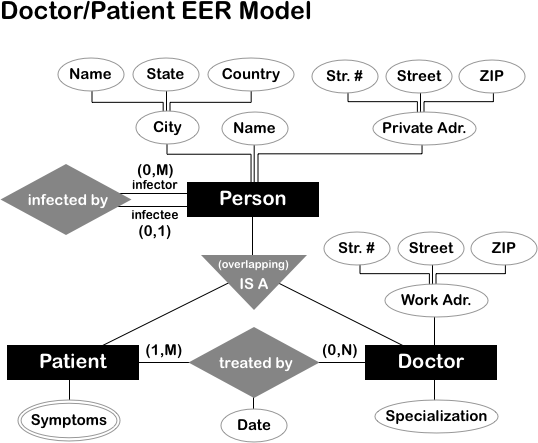
\includegraphics[scale = 0.7]{Q3b}
\vspace{2cm}

\begin{enumerate}
% \item[(10 P)] Erstellen Sie ein ER-Modell in umgekehrter (multiplikativer) Chen-Min-Max-Notation auf Grundlage der folgenden Beschreibung:\\
% \\
% Eine Person hat einen eindeutigen Login, ein Passwort, einen Namen und ein Alter. Dozierende halten Lehrveranstaltungen in einem bestimmten Semester. Studierende besuchen Lehrveranstaltungen in einem bestimmten Semester. Eine Lehrveranstaltung hat eine Nummer und einen Namen. Eine Lehrveranstaltung gehört zu genau einem Modul. Ein Modul hat einen Namen und eine Nummer. Ein Modul kann aus mehreren Lehrveranstaltungen bestehen.

% \item[(10 P)] Erstellen Sie ein ER-Modell in umgekehrter (multiplikativer) Chen-Min-Max-Notation auf Grundlage der folgenden Beschreibung:\\
% \\
% Menschen werden krank und können sich gegenseitig anstecken. Ein Patient hat einen Namen, ein Krankheitsbild und eine Privatadresse. Patienten besuchen Ärzte an einem bestimmten Tag. Wenn ein Arzt Patient ist, darf er sich nicht selbst besuchen. Ein Arzt hat einen Namen, eine Spezialisierung, eine Privatadresse und eine Dienstadresse. Die Privatadresse eines Arztes liegt immer in der selben Stadt wie seine Dienstadresse.

\item[(5 P)] Erklären Sie den Unterschied zwischen partieller und totaler Partizipation.

% \begin{itemize}
% \item Partielle Partizipation: Ein \textit{Entitätstyp A}, der \textit{partiell} an einer Relation zu einem anderen \textit{Entitätstypen B} partizipiert, kann auch ohne diesen existieren.
% \item Totale Partizipation: Ein \textit{Entitätstyp A}, der in einer \textit{totalen} Relation partizipiert, ist existenziell von einem anderen \textit{Entitätstypen B} abhängig. Der \textit{Entitätstyp A} kann nicht ohne den \textit{Entitätstypen B} existieren.
% \end{itemize}

\item[\answer]
  Partial participation of an entity type E to a relationship type R means that an entity can, but is not strictly require to, participate in the relationship. Thus there can be entities that do not participate in the relationship at all. On the other hand, total participation strictly requires that each entity of type E must participate at least once in a relationship of type R. Therefore, there exists no such entity of type E that does not participate in the relationship type R.

\end{enumerate}

\newpage

\section*{4. Aufgabe: Webserver \& JavaScript}

All code can be found in the following repository: https://github.com/jxnguyen/DBS\\

\begin{enumerate}
% \item[(10 P)] Installieren Sie einen Webserver Ihrer Wahl (zum Beispiel einen Apache httpd Webserver). Konfigurieren Sie Ihren Webserver so, dass er unter \textit{http://localhost:8050} (lokal) erreichbar ist.
\item[Install]
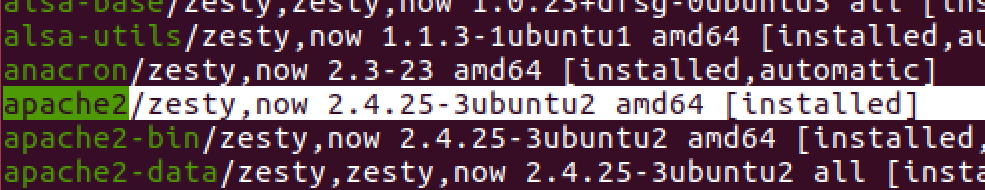
\includegraphics[scale = 0.5]{apache}\\
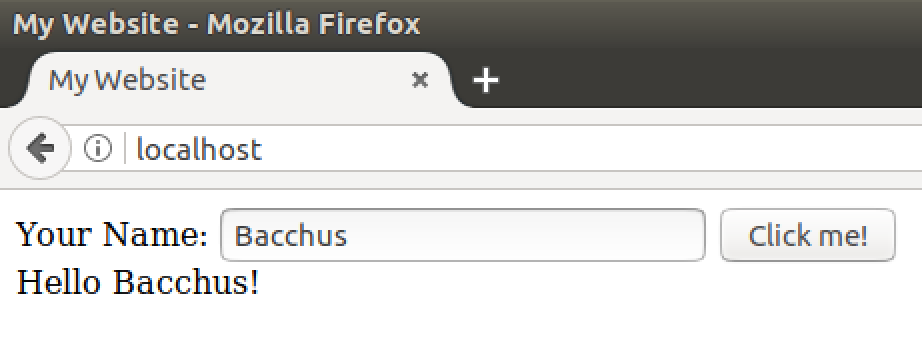
\includegraphics[scale = 0.5]{localhost}\\

% \item[(5 P)] Deployen Sie die unten stehende HTML-Seite als \textit{index.html} in Ihrem Webserver.
% \begin{verbatim}
%  1: <!doctype html>
%  2: <html>
%  3:    <head>
%  4:       <meta charset="utf-8">
%  5:       <title>Eine Webseite</title>
%  6:    </head>
%  7:    <body>
%  8:       <label for="eingabe">
%  9:          Ihr Name:
% 10:          <input id="feld" name="eingabe" />
% 11:       </label>
% 12:       <button id="knopf" type="button">
% 13:           Klick mich!
% 14:       </button>
% 15:       <div id="bereich"></div>
% 16:    </body>
% 17: </html>
% \end{verbatim}
\item[Code]
\begin{lstlisting}[language = html, breaklines = true]
  <!doctype html>
  <html>
    <head>
      <meta charset = "utf-8">
      <title>My Website</title>
      <script>
        function sayHello() {
          // get field value
          var name = document.getElementById("field").value
          // if no value entered, use default
          if (name == "") { name = "anonymous" }
          // write message in div container
          document.getElementById("container").innerHTML = "Hello " + name + "!"
        }
      </script>
    </head>

    <body>
      <label for = "input">
        Your Name: <input id = "field" name = "input"/>
      </label>
      <!-- call sayHello function when button clicked -->
      <button id ="button" type ="button", onclick ="sayHello()">
        Click me!
      </button>
      <div id = "container"></div>
    </body>
  </html>
\end{lstlisting}
% \item[(15 P)] Schreiben Sie eine JavaScript-Funktion, die im \texttt{div} Element \textit{bereich} den Text "Hallo ", ergänzt durch den Text aus dem Eingabefeld \textit{feld} ausgibt, sobald der Knopf \textit{knopf} gedrückt wird. Wenn kein Text im Eingabefeld \textit{feld} steht, soll "Hallo Unbekannter!" im \texttt{div} Element \textit{bereich} ausgegeben werden.
%
% Lesen Sie hierzu: \textit{https://www.w3schools.com/js/default.asp}
%
% Ergänzen Sie das \textit{index.html} Dokument um Ihre Javascript-Funktion. Drucken Sie Ihren Quellcode und fügen Sie ihn Ihrer Abgabe hinzu.
\end{enumerate}


\end{document}
